\section{Frozen predictions and their tests}\label{sec:frozen}

The tests above check claims made before them. This section lists the tests whose outcomes are pending in this version, with the predictions frozen for them (Table~\ref{tab:frozen}). Each prediction was committed under the tag named, with its scoring rule frozen alongside, before any of its results was read by the agents that made it; Table~\ref{tab:timeline-r11} gives the GitHub push times recorded so far, and the others are pending. Each registered test has a FILLED registration committed and tagged before its first job; the GitHub push times of these registrations are pending (Table~\ref{tab:ledger}). Every outcome will be reported against these rules, misses included.

\paragraph{GPU generation.} The H200 cell repeats the 300k SGLang cell on one H200 NVL. Its only inputs beyond the A100 cell are its E0a measurements: the all-miss token rate fixes the speed factor $s=2.742$ of Proposition~\ref{prop:nb}(c), the turns-based $\lref$ (0.194\sps) is the denominator of the peak ratio, and the 64-to-32-session ratio of all-miss token rates sets one cost variant. The model predicts that the peak ratio falls to 1.92 while the all-miss onset moves out to 41.3 sessions (Fig.~\ref{fig:fpscale}); the frozen refutation rules are a peak ratio of 2.4 or more, a hit fraction below 0.5 at $n=32$, or one of 0.5 or more at $n=48$. Three extra closed runs at $n=36$, 44 and 52 bracket the predicted crossing at $n=37.3$, and a 600k-token H200 cell, with the 600k A100 cell of the pool sweep, completes a two-by-two test of Proposition~\ref{prop:scaling}. KAIROS shows qualitatively that a slower clock tips a fixed arrival rate into thrashing~\citep{yuan2026kairos}, and VAMP locates KV capacity boundaries on H100 and H200 GPUs~\citep{kim2026vamp}; the new parts would be the measurement in units of $\lmiss$ and the opposite movement of the onset and the peak ratio. The session that operated the H200 cell saw its closed-curve values for $n\le32$ before the freeze and showed them to the first author; the agents that derived and froze the model did not see them. These values include the region of the predicted peak ($n\approx32.5$), so the peak-ratio rule ($\omega\ge2.4$), the hit fraction at the peak and hit$(32)$ are not blind to the first author; only $n\ge36$ and the from-empty edge were blind to everyone. The edge is scored on the original E0b runs (jobs 17168377--82); four reseeds (17169668--71, at 1.3 and 1.4 $\lref$) were added after those runs had been read and are reported separately.

\paragraph{Pools and a second model.} The pool sweep repeats Stage~C and E0b on the A100 with pools of 150k and 600k tokens, with no fitted parameter; its 150k from-empty edge discriminates between F2 and a second edge criterion, which predict 1.09 and 1.47 $\lref$. The Llama-3.1-8B cell keeps the engine, the GPU and the 300k pool. The model's a priori costs for it come from published architecture ratios; the pool part $M/E_S=27.8$ does not depend on the model's speed; and once the cell's all-miss rate is measured, every predicted quantity is read from a frozen table indexed by the speed factor.

\paragraph{The basin.} Two registered BURST-only tests at 1.65 $\lref$ on the 300k pool vary the burst size: B1 with 25 and 100 sessions and B2 with 40, 50 and 60. The theory predicts whether a run is stuck, with a hit fraction below 0.2 over the evaluation window; it does not model the slope test of the registered trap rule, which is co-primary only for B1's 100-session cell. The model's critical fresh burst is 53.4 sessions, and its per-seed probabilities of a stuck run are 0.04, 0.14, 0.55 and 1.0 for 25, 40, 50 and 60 or more sessions; the stationary-composition estimate, 21.3 sessions, would have 40 stuck. B2's frozen rule calls the boundary bracketed if 40 stays good and 60 is stuck, each in at least two of three seeds. The critical burst and the stationary estimate are both defined at $n_2$, where $\mu(n)$ does not determine them (\S\ref{sec:fp-weak}), so B2 tests the heuristic F3, not a consequence of the propositions. A from-empty test with fresh seeds (3, 4 and 5, at 2.0 and 2.5 $\lref$) asks whether the measured edge depends on E0b's single arrival seed: the simulator predicts that it does, with 2.5 $\lref$ stable in all three, while F2 makes 2.5 $\lref$ unstable with probability 0.69 per seed.

\paragraph{Rescue and shedding.} Two registered tests engage a cap inside an established trap and release it once the gate has been empty for 300\,s: R1 on the 300k pool (cap 20 at 1800\,s, at 1.35 and 1.65 $\lref$) and R4 with the native pool (cap 64 at 2100\,s, at 4.0 $\lref$). The simulator and the model both predict rescue. At the fluid rate of the paused sessions, whose next turns miss, the model predicts release at 3830, 4360 and 5040\,s ($\pm15\%$; with F1, 3920, 4480 and 5250\,s); it predicts release before the 7200\,s deadline only if those sessions complete at no less than 32, 42 and 51\% of that rate. The gate pauses sessions only at tool-call boundaries and defers work rather than dropping it. Pausing whole programs at tool boundaries is ThunderAgent's and NVIDIA Dynamo's mechanism~\citep{kang2026thunderagent,dhanani2026dynamo}; CONCUR cuts its window of active agents multiplicatively when it detects thrashing (hit rate below 0.2 with KV usage above 0.5) to exit that regime, and MISA-T contracts its cap temporarily on a confirmed hit-rate decline, both in closed or bounded populations~\citep{chen2026concur,hong2026misat}; KAIROS bounds aggregate context and, when bursty arrivals have already broken the bound, defers new agents and boosts the clock, but reports no recovery from an established trap~\citep{yuan2026kairos}; inhibiting new traffic until a bistable channel returns to its lower state was proposed by Carleial and Hellman~\citep{carleial1975bistable}, and shedding load is the usual response in production~\citep{huang2022metastable}. The new parts would be a rescue from an established trap under open arrivals, a measured test that the good state persists after the cap is released, and a rescue condition and release times frozen beforehand. The SHED test measures the alternative: arrivals stop for $\tau=600$ or 3600\,s from 1800\,s, refusing about $\lambda\tau=58$ or 348 sessions, against none for the cap.

\paragraph{Causes.} TOOLSLOW lengthens every tool call that starts in $[1200,2100)$\,s by $\delta=10$ or 30\,s in the NOBURST arm at 1.35 $\lref$, a trigger that involves neither a burst nor a lowered clock. Its registered rule expects the 10\,s slowdown to leave the engine good and the 30\,s slowdown to leave it stuck, each in at least two of three seeds. In the frozen model (pred2) the slowdown acts through capacity and population: for $\delta$ above 13.7\,s the slowed curve's peak lies below $\lambda=0.0966$\sps, so it has no good state (at $\delta=30$\,s the peak is the all-miss level $\mu_b=0.0718$\sps); at $\delta=30$\,s the population reaches 46.9 sessions by 2100\,s, above $n_2=32.2$, while at $\delta=10$\,s it reaches 21.5, near the slowed curve's good state (21.8 sessions, against 8.5 without the slowdown). A pass would show that a temporary increase in tool latency, with no burst, can trigger the trap; it would not separate the longer gap from the capacity loss and the larger population that come with it. LPM-INF disables stock LPM's 128-request fallback (\S\ref{sec:grid}); the simulator predicts that LPM then avoids the all-miss collapse on the two seeds on which stock LPM collapsed, in a partial-hit state that the registered rule still calls trapped.

\begin{figure*}[t]\centering
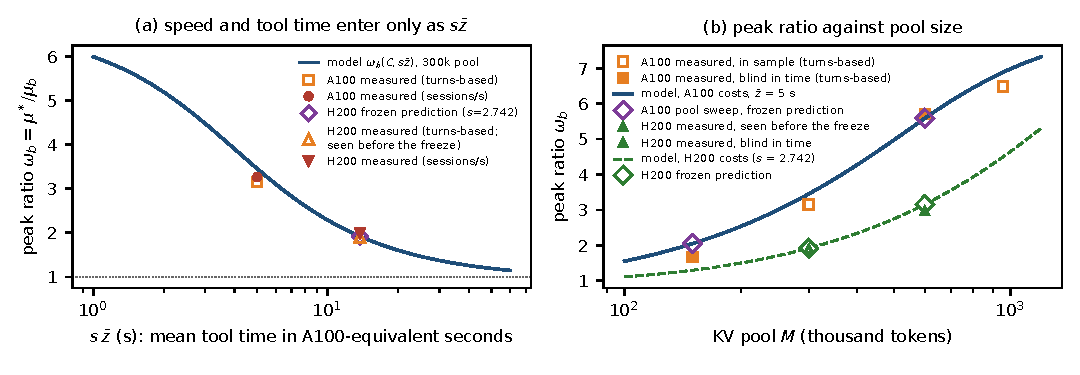
\includegraphics[width=\textwidth]{figs/fig9_theory_scaling.pdf}
\caption{Frozen predictions of the peak ratio $\omega=\mu^*/\mu_b$ (fluid model, in model units). (a) Against $s\bar z$, the mean tool time in A100-equivalent seconds, for the 300k pool (Proposition~\ref{prop:scaling}); squares and dot: the A100, measured (turns-based, sessions/s); diamond: the H200 prediction ($s=2.742$). (b) Against the pool size, A100 costs, $\bar z=5$\,s; squares: measured cells (turns-based); diamonds: the pool-sweep predictions. Outcomes are pending. Table~\ref{tab:frozen} quotes the primary predictions (F1, against $\lref$), which are lower than the plotted fluid values by 0.1\% (H200) to 8.6\% (150k).}\label{fig:fpscale}
\end{figure*}

\begin{table*}[tp]
\centering\footnotesize
\caption{Frozen predictions and their tests. Each prediction was committed under the tag named before any of its results was read by the agents that made it (for the H200 exception see its row); scoring rules and tolerances were frozen with it (\fpath{notes/THEORY_r13_scoring.md} for the theory; the registration file or \fpath{configs/r11_*_predict.yaml} otherwise). ``Theory'': the model of \S\ref{sec:fp}, tag \texttt{r13-theory-pred} (\S\ref{sec:fp-val}), files under \fpath{results/theory/merged/}; ``pred2'': the same model, tag \texttt{r13-theory-pred2} (commit \texttt{cfa7712}, pushed 04:20:20 CDT, before the first B2, TOOLSLOW or SHED job by its freeze record; files under \fpath{results/theory/pred2/} at that tag). ``Simulator'': the calibrated simulator of \S\ref{sec:sim}. $\omega=\mu^*/\lref$ (turns-based), with $\lref$ the cell's measured E0a rate (pool sweep: the A100 300k value, 0.0715\sps; H200 600k: the H200 300k value, 0.194\sps; Llama: the model's a priori $\lmiss$); hit is the fraction of all turns of a closed run that hit (first turns always miss, so at most 0.932), the Stage~C estimator; stuck means a hit fraction below 0.2 over the evaluation window.}\label{tab:frozen}
\setlength{\tabcolsep}{3pt}
\begin{tabular}{@{}>{\raggedright\arraybackslash}p{2.9cm} >{\raggedright\arraybackslash}p{8.1cm} >{\raggedright\arraybackslash}p{3.6cm} >{\raggedright\arraybackslash}p{2.3cm}@{}}
\toprule
Test & Frozen prediction & Source & Outcome\\
\midrule
H200 NVL, SGLang, 300k pool: curve & $\omega=1.92$ (band 1.65--1.92 over the five cost variants; fluid 1.66--1.96; A100: 3.27 predicted, 3.15 measured); all-miss onset $n_b=41.3$ (A100: 32.7); 0.5-hit crossing at $n=37.3\pm3$; hit 0.67 at the peak, $n\approx32.5$. Refuted if $\omega\ge2.4$, hit$(32)<0.5$ or hit$(48)\ge0.5$; the first two are not blind to the first author, who had seen $n\le32$. & theory, \fpath{h200_300k*.json}; $s=2.742$ fitted to the H200's all-miss token rate & \pending{H200 Stage C}\\
\addlinespace[0.3pt]
H200: cliff bracket, $n=36$, 44, 52 & Hit, fluid: 0.56 at $n=36$ (variants 0.52--0.57), 0 at 44 and 52; F1: 0.53 (0.50--0.53), 0.08, 0.002 (from the frozen curves, not the freeze record) & theory, \fpath{h200_300k*.json} (closed curve) & \pending{Stage C 17169612--14}\\
\addlinespace[0.3pt]
H200: from-empty edge & F2 edge $1.39\,\lref$ (1.24--1.40 over the cost variants); scored on the original E0b runs 17168377--82, not the later reseeds & theory, \fpath{h200_300k*.json} & \pending{H200 E0b}\\
\addlinespace[0.3pt]
H200 NVL, 600k pool & pred2 (jobs submitted at about 03:15 CDT, held until 05:00): $n_b=69.9$, as Proposition~\ref{prop:nb}(c) gives from the 600k A100 onset and $s$; $\omega=3.20$ (fluid 3.27); crossing 66.6; F2 edge $2.57\,\lref$ & pred2, \fpath{h200_600k.json} & \pending{Stage C 17169672--80, E0b 17169682--87}\\
\addlinespace[0.3pt]
Llama-3.1-8B, SGLang, A100, 300k & Theory, a priori: $M/E_S=27.8$ for any speed, $n_b=32.0$, crossing 30.9, $\omega=3.37$, edge $2.46\,\lmiss$; after the cell's $\lmiss$ is measured, every quantity comes from the frozen speed table. Refuted if the crossing lies outside the table's value $\pm3$, or $\mu(48)$ is within 10\% of the peak. Simulator, costs scaled to the measured all-miss rate: peak at $n=20$, $\omega=3.52$, crossing 30.6, edge $2.5\,\lmiss$, paired test passes at every candidate rate. & theory, \fpath{llama31_8b_300k*.json}; simulator, tag \texttt{r12-llama31-\allowbreak predictions-frozen}, \fpath{notes/PREDICTIONS_llama31.md} & \pending{Stage C 17166814--16, E0b 17169565--70; registration pending}\\
\addlinespace[0.3pt]
Pool sweep, SGLang, A100, 150k and 600k & $\omega=1.87$ and 5.47; $n_b=18.3$ and 61.2; crossing 16.9 and 60.0; F2 edge 1.09 and $4.53\,\lref$ (second criterion 1.47 and 4.82). Refuted if $\omega\ge2.5$ or hit$(24)\ge0.5$ at 150k, or $\omega<4.5$ or hit$(48)<0.5$ at 600k. No fitted parameter. & theory, \fpath{a100_pool150k.json}, \fpath{a100_pool600k.json} & \pending{Stage C 17168864--69, E0b 17168870--81}\\
\addlinespace[0.3pt]
Fresh-seed E0b, 300k, seeds 3--5, 2.0 and 2.5 $\lref$ & Simulator: stable in 3 of 3 at both rates, so the seed-0 bracket is not replicated. Theory (F2): unstable with probability 0.15 and 0.69 per seed. & simulator, tag \texttt{r11-basin-reg}; theory, \fpath{a100_300k.json} & \pending{E0F runs}\\
\addlinespace[0.3pt]
Basin B1, 300k, 1.65 $\lref$, bursts 25, 100 (registered) & Simulator: pass (100 stuck and trapped, 25 good, each in 3 of 3). Theory: stuck with probability 1.000 and 0.042 per seed; pass with probability 0.995. & registration and simulator, tag \texttt{r11-basin-reg}; theory, \fpath{b1_basin_300k.json} & \pending{B1 verdict}\\
\addlinespace[0.3pt]
Basin B2, bursts of 40, 50 and 60 (registered) & Theory: stuck with probability 0.139, 0.547 and 1.000 per seed (critical fresh burst 53.4). Rule: bracketed if 40 is good and 60 stuck, each in at least 2 of 3 seeds. pred2, conditioning on each seed's burst: the rule holds with probability 0.66 (bands 0.23--0.88; 0.94 for average bursts) & registration, tag \texttt{r14-basin2-reg}; theory, \fpath{b1_basin_300k.json}; pred2, \fpath{b2_basin.json} & \pending{B2 verdict}\\
\addlinespace[0.3pt]
Rescue R1, 300k, cap 20 engaged at 1800\,s, 1.35 and 1.65 $\lref$ (registered) & Simulator: rescued in 20 of 20 seeds at both rates, release at 3490--5830 and 4050--6050\,s. Theory: rescued, release at 3830 and 4360\,s ($\pm15\%$), relapse probability 0.002 and 0.025; the 7200\,s deadline is missed if the paused sessions complete below 32\% and 42\% of their fluid rate. & registration, tag \texttt{r11-rescue-reg}; simulator, tag \texttt{r11-rescue-pred}; theory, \fpath{r1_rescue_300k.json} & \pending{R1 verdict}\\
\addlinespace[0.3pt]
Rescue R4, native pool, cap 64 at 2100\,s, 4.0 $\lref$ (registered) & Simulator: rescued in 16 of 20 seeds, seeds 0--2 rescued; the engage time was moved from 2400\,s (13 of 20) after that prediction and before any rescue run. Theory: rescued, release at 5040\,s ($\pm15\%$); the 7200\,s deadline is missed if the paused sessions complete below 51\% of their fluid rate. & as R1; theory, \fpath{r4_rescue_native.json} & \pending{R4 verdict}\\
\addlinespace[0.3pt]
SHED, 300k, BURST at 1.35 $\lref$, arrivals stopped for $\tau$ from 1800\,s (registered) & Rule: $\tau=600$\,s stuck and $\tau=3600$\,s good, in 2 of 2 seeds; sessions refused (about 58 and 348) reported against none for the cap. Simulator: a full stop from 1800\,s lasting 3600\,s rescued 10 of 10, dropping 328--378 sessions; one lasting 3000\,s rescued 8 of 10. pred2: the shortest rescuing stop lasts 1795\,s (Eq.~\eqref{eq:fluid} from RR's 161 sessions at 1800\,s; RR alone: 1928\,s); $\tau=600$\,s stuck (1.00), $\tau=3600$\,s good (0.998); the rule holds with probability 0.997. & registration, tag \texttt{r14-extra-reg}; simulator, tag \texttt{r11-rescue-pred}; pred2, \fpath{shed.json} & \pending{SHED verdict}\\
\addlinespace[0.3pt]
TOOLSLOW, 300k, NOBURST, 1.35 $\lref$, $Z+\delta$ in $[1200,2100)$\,s (registered) & Rule: $\delta=10$\,s good and $\delta=30$\,s stuck, each in at least 2 of 3 seeds. pred2: $\delta=10$\,s good with probability 0.71 per seed, $\delta=30$\,s stuck (1.00); the rule holds with probability 0.80 (band 0.63); critical $\delta$ 16.8\,s (fluid), 16.4\,s (stochastic). & registration, tag \texttt{r14-extra-reg}; pred2, \fpath{toolslow.json} & \pending{TOOLSLOW verdict}\\
\addlinespace[0.3pt]
LPM-INF, 300k, BURST, 1.65 $\lref$, no 128-request fallback (exploratory) & Simulator: no collapse on seeds 0--2 (token hit fraction 0.08--0.10), including seeds 0 and 1, on which stock LPM collapsed; the frozen rule reads this as the fallback causing that collapse, and the registered rule still calls each run trapped. & tag \texttt{r11-lpminf-pred}, \fpath{configs/r11_lpminf_predict.yaml} & \pending{LPM-INF runs}\\
\bottomrule
\end{tabular}
\end{table*}
